
\documentclass[border=10pt, 12pt]{standalone}
\usepackage[svgnames]{xcolor}
\usepackage{amsmath}
\usepackage{pgfplots}
\pgfplotsset{compat=newest}
\usepackage[sfdefault]{FiraSans}
\usepackage{FiraMono}
\renewcommand*\familydefault{\sfdefault}
\begin{document}
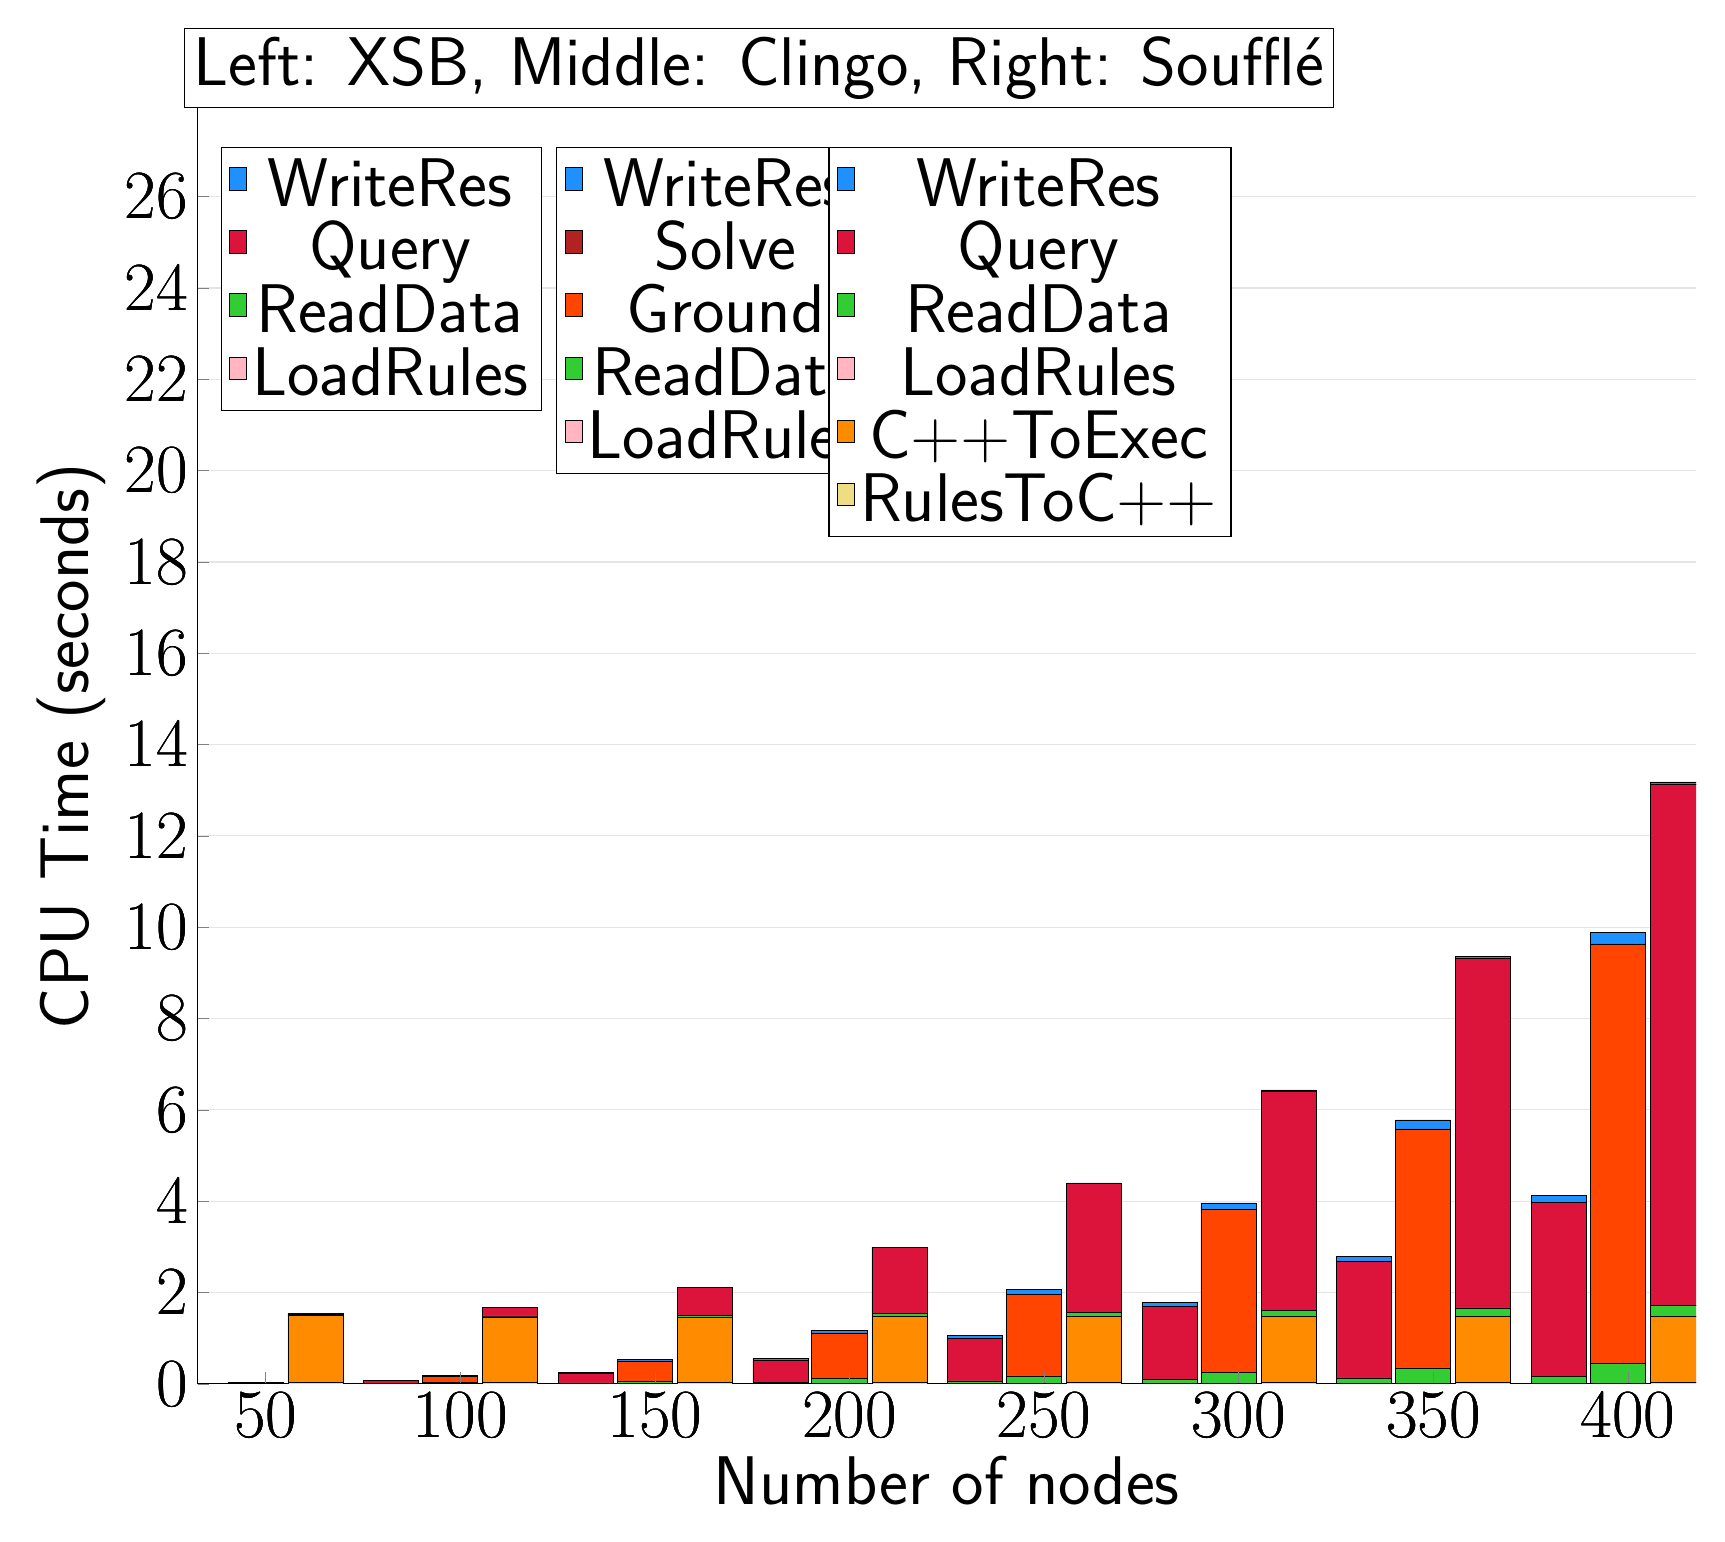
\begin{tikzpicture}
	\begin{axis}[bar shift=-25pt,
			ybar stacked,
			width=1.7\textwidth,
			bar width=0.7cm,
			ymajorgrids, tick align=inside,
			major grid style={draw=gray!20},
			xtick=data,
			ymin=0, ymax=27.933910000000004,
			axis x line*=bottom,
			axis y line*=left,
			enlarge x limits=0.05,
			legend style={
					at={(0.23, 0.97)},
					anchor=north east,
					legend columns=1,
					font=\Huge,
				},
			ylabel={CPU Time (seconds)},
			xlabel={Number of nodes},
			label style={font=\Huge},
			tick label style={font=\Huge},
		]
		\addlegendimage{fill=DodgerBlue, draw=black, line width=0.2pt}
		\addlegendentry{WriteRes}
		\addlegendimage{fill=Crimson, draw=black, line width=0.2pt}
		\addlegendentry{Query}
		\addlegendimage{fill=LimeGreen, draw=black, line width=0.2pt}
		\addlegendentry{ReadData}
		\addlegendimage{fill=LightPink, draw=black, line width=0.2pt}
		\addlegendentry{LoadRules}
		\addplot +[fill=LightPink, draw=black, line width=0.2pt] coordinates {
				(50, 0.0005436999999999999)
				(100, 0.0006297)
				(150, 0.0006088999999999999)
				(200, 0.0006082000000000001)
				(250, 0.0006123999999999998)
				(300, 0.0006215000000000003)
				(350, 0.0006266999999999999)
				(400, 0.0006372000000000003)
			};
		\addplot +[fill=LimeGreen, draw=black, line width=0.2pt] coordinates {
				(50, 0.0023761999999999998)
				(100, 0.0088507)
				(150, 0.0206731)
				(200, 0.0383251)
				(250, 0.061571799999999996)
				(300, 0.0910103)
				(350, 0.12799129999999997)
				(400, 0.1706672)
			};
		\addplot +[fill=Crimson, draw=black, line width=0.2pt] coordinates {
				(50, 0.0077931)
				(100, 0.059859300000000004)
				(150, 0.20364539999999995)
				(200, 0.48165009999999997)
				(250, 0.9390012999999999)
				(300, 1.6043246)
				(350, 2.5467262000000006)
				(400, 3.8088134000000005)
			};
		\addplot +[fill=DodgerBlue, draw=black, line width=0.2pt] coordinates {
				(50, 0.0022654999999999997)
				(100, 0.0090485)
				(150, 0.022953)
				(200, 0.03450349999999998)
				(250, 0.0557735)
				(300, 0.07931240000000002)
				(350, 0.1196857)
				(400, 0.1429398)
			};
	\end{axis}

	\begin{axis}[bar shift=-3.7pt,
			ybar stacked,
			width=1.7\textwidth,
			bar width=0.7cm,
			ymajorgrids, tick align=inside,
			major grid style={draw=none},
			xtick=data,
			ymin=0, ymax=27.933910000000004,
			axis x line*=none,
			axis y line*=none,
			enlarge x limits=0.05,
			legend style={
					at={(0.454, 0.97)},
					anchor=north east,
					legend columns=1,
					font=\Huge,
				},
			label style={font=\Huge},
			tick label style={font=\Huge},
		]
		\addlegendimage{fill=DodgerBlue, draw=black, line width=0.2pt}
		\addlegendentry{WriteRes}
		\addlegendimage{fill=FireBrick, draw=black, line width=0.2pt}
		\addlegendentry{Solve}
		\addlegendimage{fill=OrangeRed, draw=black, line width=0.2pt}
		\addlegendentry{Ground}
		\addlegendimage{fill=LimeGreen, draw=black, line width=0.2pt}
		\addlegendentry{ReadData}
		\addlegendimage{fill=LightPink, draw=black, line width=0.2pt}
		\addlegendentry{LoadRules}
		\addplot +[fill=LightPink, draw=black, line width=0.2pt] coordinates {
				(50, 0.0)
				(100, 0.0)
				(150, 0.0)
				(200, 0.0)
				(250, 0.0)
				(300, 0.0)
				(350, 0.0)
				(400, 0.0)
			};
		\addplot +[fill=LimeGreen, draw=black, line width=0.2pt] coordinates {
				(50, 0.009999999999999997)
				(100, 0.030000000000000006)
				(150, 0.06000000000000001)
				(200, 0.11200000000000002)
				(250, 0.173)
				(300, 0.252)
				(350, 0.34700000000000003)
				(400, 0.4490000000000001)
			};
		\addplot +[fill=OrangeRed, draw=black, line width=0.2pt] coordinates {
				(50, 0.018000000000000006)
				(100, 0.12999999999999998)
				(150, 0.43899999999999995)
				(200, 1.001)
				(250, 1.7810000000000001)
				(300, 3.562)
				(350, 5.225)
				(400, 9.169)
			};
		\addplot +[fill=FireBrick, draw=black, line width=0.2pt] coordinates {
				(50, 0.0020000000000000005)
				(100, 0.0)
				(150, 0.0010000000000000009)
				(200, 0.0050000000000000044)
				(250, 0.007000000000000029)
				(300, 0.008000000000000009)
				(350, 0.011999999999999744)
				(400, 0.01700000000000017)
			};
		\addplot +[fill=DodgerBlue, draw=black, line width=0.2pt] coordinates {
				(50, 0.0020000000000000005)
				(100, 0.020000000000000018)
				(150, 0.036999999999999963)
				(200, 0.05999999999999996)
				(250, 0.09900000000000012)
				(300, 0.14300000000000002)
				(350, 0.1960000000000004)
				(400, 0.25899999999999945)
			};
	\end{axis}

	\begin{axis}[bar shift=18pt,
			ybar stacked,
			width=1.7\textwidth,
			bar width=0.7cm,
			ymajorgrids, tick align=inside,
			major grid style={draw=none},
			xtick=data,
			ymin=0, ymax=27.933910000000004,
			axis x line*=none,
			axis y line*=none,
			enlarge x limits=0.05,
			legend style={
					at={(0.69, 0.97)},
					anchor=north east,
					legend columns=1,
					font=\Huge,
				},
			label style={font=\Huge},
			tick label style={font=\Huge},
		]
		\addlegendimage{fill=DodgerBlue, draw=black, line width=0.2pt}
		\addlegendentry{WriteRes}
		\addlegendimage{fill=Crimson, draw=black, line width=0.2pt}
		\addlegendentry{Query}
		\addlegendimage{fill=LimeGreen, draw=black, line width=0.2pt}
		\addlegendentry{ReadData}
		\addlegendimage{fill=LightPink, draw=black, line width=0.2pt}
		\addlegendentry{LoadRules}
		\addlegendimage{fill=DarkOrange, draw=black, line width=0.2pt}
		\addlegendentry{C++ToExec}
		\addlegendimage{fill=LightGoldenrod, draw=black, line width=0.2pt}
		\addlegendentry{RulesToC++}
		\addplot +[fill=LightGoldenrod, draw=black, line width=0.2pt] coordinates {
				(50, 0.031000000000000007)
				(100, 0.030000000000000006)
				(150, 0.030000000000000006)
				(200, 0.030000000000000006)
				(250, 0.030000000000000006)
				(300, 0.030000000000000006)
				(350, 0.030000000000000006)
				(400, 0.030000000000000006)
			};
		\addplot +[fill=DarkOrange, draw=black, line width=0.2pt] coordinates {
				(50, 1.4649999999999999)
				(100, 1.4369999999999998)
				(150, 1.4329999999999998)
				(200, 1.4469999999999998)
				(250, 1.4439999999999997)
				(300, 1.4439999999999995)
				(350, 1.453)
				(400, 1.454)
			};
		\addplot +[fill=LightPink, draw=black, line width=0.2pt] coordinates {
				(50, 1.11e-05)
				(100, 1.02e-05)
				(150, 1.02e-05)
				(200, 0.0)
				(250, 0.0)
				(300, 0.0)
				(350, 0.0)
				(400, 0.0)
			};
		\addplot +[fill=LimeGreen, draw=black, line width=0.2pt] coordinates {
				(50, 0.005443600000000001)
				(100, 0.0203258)
				(150, 0.0410564)
				(200, 0.0647587)
				(250, 0.09538469999999999)
				(300, 0.13409449999999998)
				(350, 0.1778328)
				(400, 0.23472890000000005)
			};
		\addplot +[fill=Crimson, draw=black, line width=0.2pt] coordinates {
				(50, 0.0322895)
				(100, 0.1887387)
				(150, 0.6043478)
				(200, 1.4434140000000002)
				(250, 2.814502)
				(300, 4.803262)
				(350, 7.660176999999999)
				(400, 11.42133)
			};
		\addplot +[fill=DodgerBlue, draw=black, line width=0.2pt] coordinates {
				(50, 0.0009866999999999999)
				(100, 0.0028780000000000003)
				(150, 0.0062959)
				(200, 0.0110188)
				(250, 0.017276600000000003)
				(300, 0.0247944)
				(350, 0.0337603)
				(400, 0.04420929999999999)
			};
	\end{axis}


	\node[anchor=south, draw, fill=white] at (rel axis cs:0.42,1) {\Huge Left: XSB, Middle: Clingo, Right: Soufflé};
\end{tikzpicture}
\end{document}
